%% Source: https://github.com/tias/constraint-solving-course
%% Licensed under CC BY-NC-SA 4.0: https://creativecommons.org/licenses/by-nc-sa/4.0/
%% You may share and adapt this for non-commercial use,
%% with attribution and under the same license.

\documentclass{cons-beamer}

\begin{document}

\titleFrame{
	L07: Solving technologies and encodings, part 2
}{
	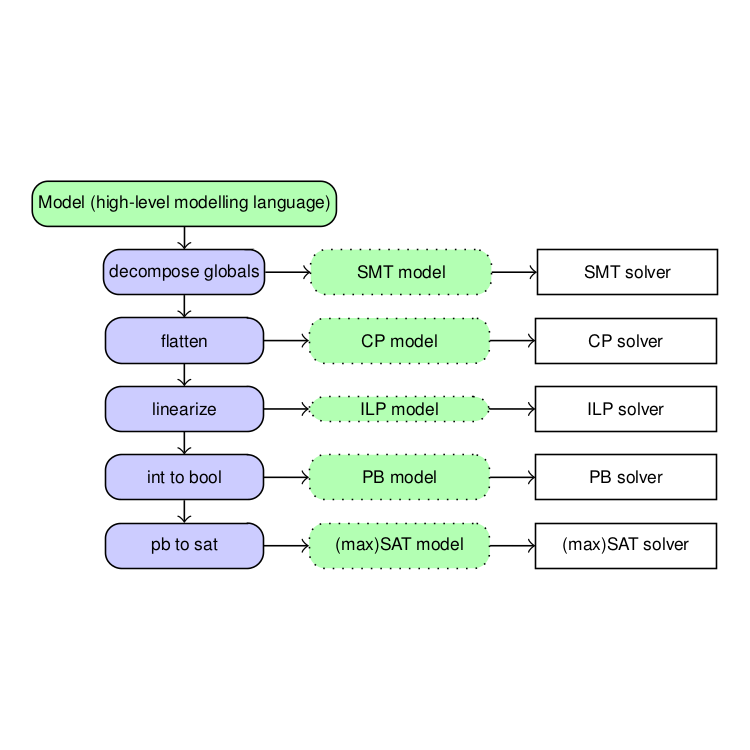
\includegraphics[height=42mm, trim=5pt 50pt 0 55pt, clip]{images/ch6-logo.png}
}{
	Partly based on slides from Pierre Flener, Ambros Gleixner and Jakob Nordstr\"om
}

\begin{frame}{Recap, goal of the lecture}
	\textbf{Part 2} of solving technologies and encodings.
	\vfill

	Part 1 covered SMT, decomposing global constraints, and CP solving (search + propagation).
	\vfill

	This lecture: flatten nested expressions; ILP (+ linearisation); PB; int$\to$bool encodings; SAT/CDCL; PB$\to$SAT; choosing a technology.
	\vfill
	\pause

	Still the same goals: \vfill
	\begin{itemize}
		\item to understand advantages and limitations of each technology; \vfill
		\item to help you choose a technology for a particular model; \vfill
		\item to help you encode and adapt a model to a particular technology.
	\end{itemize}
\end{frame}


\subsection*{Transformation: flatten}
\begin{frame}{Overview}
	\begin{tikzpicture}[scale=0.7, every node/.style={transform shape}, node distance=0.5cm]
		\waterfall[flatten]
	\end{tikzpicture}
\end{frame}

\begin{frame}{From CP Language to CP Solver: primitive constraints}
	A CP solver accepts as input a number of \textit{primitive constraints}, that each will have a propagator that can do \inference{inference}.
	\vfill
	
	Example primitive constraints, note their arguments are \textit{variables}:
	\begin{align*}
		& a \lor b \\
		& x \neq y \\
		& x + y \geq 2 \\
		& x + 2 \cdot y \neq 3 \\
		&\cons{AllDifferent}{x,y,z} \\
		&\cons{CountEq}{[x,y,z], 0, r} \\
	\end{align*}
\end{frame}


\begin{frame}{From CP Language to CP Solver: primitive constraints}
	A CP solver accepts as input a number of \textit{primitive constraints}, that each will have a propagator that can do \inference{inference}.
	\vfill
	
	Also primitive for many CP solvers: one level of reification (Boolean decision variable on left-hand-side):
	\begin{align*}
		&b = (x = 0) \\
		&b \rightarrow x \neq 3 \\
		&b \rightarrow (y + z \leq 3) \\
		&b \rightarrow (5\cdot y - 2\cdot z \leq 3) \\
	\end{align*}
	
\end{frame}

\begin{frame}{From CP Language to CP Solver: non-primitive constraints}
	Example \textbf{nested} constraints, not primitive because their arguments contain \textit{\textcolor{blue}{sub-expressions}}:
	\begin{align*}
		& \neg (\textcolor{blue}{a \lor b}) \\
		& \neg (\textcolor{blue}{x > y}) \\
		& a \rightarrow (\textcolor{blue}{b \lor c})\\
		%& a \lor (x \neq y) \\
		& a \lor (\textcolor{blue}{x + y \geq 2}) \\
		& x + (\textcolor{blue}{y \cdot z}) \geq 0 \\
		& (\textcolor{blue}{a \lor b}) = (\textcolor{blue}{x = 0}) \\
		& x + 3\neq \textcolor{blue}{\cons{Count}{[y,z,q], 0}} \\
		%& \cons{Count}{[x,y,z], 0} + q \geq 2 \\
		&\cons{AllDifferent}{\textcolor{blue}{x+2},\textcolor{blue}{y-1},z} \\
		&\cons{CountEq}{[\textcolor{blue}{x+2},\textcolor{blue}{y-1},z], 0, \textcolor{blue}{r+2\cdot s}} \\
		%& (\neg (a \lor b)) \rightarrow (y + z \leq 3) \\
	\end{align*}
\end{frame}

\begin{frame}{From CP Language to CP Solver: negation}
	Assume all unsupported global constraints have been decomposed already.
	
	\textbf{Eliminating negation}
	
	Negation $\neg (E)$ is not a primitive constraint of CP solvers, because it can be \textit{eliminated}, by applying a set of rewrite rules over Boolean expressions:
	
	\begin{itemize}
		\item $\neg b$ \quad with $b$ a Boolean variable is the only allowed negated expression. Recall that $b$ and $\neg b$ are called the \textit{literals} of Boolean variable $b$.
		\item $\neg (x ~\text{CMP}~ y)$, \quad with CMP a comparison relation, has standard mathematical negation rules: $= ~\Leftrightarrow~ \neq,\quad > ~\Leftrightarrow~ \leq,\quad < ~\Leftrightarrow~ \geq$.
		\item $\neg (\neg (E)) \Leftrightarrow E$.
	\end{itemize}
	\pause
	\vfill
	
	The next two can now be applied recursively to eliminate negated expressions.
	\begin{itemize}
		\item $\neg (E_1 \land E_2)$, \quad by DeMorgan's law is equivalent to $(\neg E_1) \lor (\neg E_2)$.
		\item $\neg (E_1 \lor E_2)$, \quad also by DeMorgan's law equivalent to $(\neg E_1) \land (\neg E_2)$. Likewise $\neg (E_1 \rightarrow E_2)$ is equivalent to $E_1 \land (\neg E_2)$ because $(E_1 \rightarrow E_2) \Leftrightarrow ((\neg E_1) \lor E_2)$.
	\end{itemize}
	
\end{frame}


\begin{frame}{From CP Language to CP Solver: flattening}	
	\defined{Flattening} is the process of replacing subexpressions by fresh auxiliary variables, with an additional constraint that enforces the 
	variable to equal the subexpression.
	\vfill
	
	\textbf{Numeric subexpressions}\\
	Create a new auxiliary decision variable with the same bounds as the subexpression and enforce equality:\\
	Example: $x + (\textcolor{blue}{y \cdot z}) \geq 0 ~\Leftrightarrow~ x + \textcolor{blue}{r} \geq 0 \land (\textcolor{blue}{r = y \cdot z})$
	\vfill
	\pause
	
	\textbf{Boolean subexpressions}\\
	Example: $x + \textcolor{blue}{\Iverson{y > z}} = 3  ~\Leftrightarrow~ x + \textcolor{blue}{e} = 3 \land (\textcolor{blue}{e \leftrightarrow y > z})$.
	
	Special cases: $x + \textcolor{blue}{\Iverson{y > z}} \boldsymbol{\geq} 3$ and $a \lor \textcolor{blue}{(y > z)}$ only care about the truthness of $(y > z)$, so $\textcolor{blue}{e \rightarrow y > z}$ is sufficient.
	
	Likewise, $x + \textcolor{blue}{\Iverson{y > z}} \boldsymbol{\leq} 3$ only cares about falseness, so $\textcolor{blue}{e \leftarrow y > z}$ is sufficient.
	\vfill
	\pause
	
	\textbf{Common subexpression elimination:} if a subexpression already has an auxiliary variable created for it, reuse that.
	
\end{frame}


\begin{frame}{From CP Language to CP Solver: simplification and normalisation}
	
	If we can \textbf{avoid creating auxiliary variables}, we should: more compact formulation, and the solver can reason more directly on the original variables.
	\vfill
	
	We can do this by \textbf{simplifying} and \textbf{normalizing} expressions, before flattening their subexpressions.
	
	\begin{itemize}
		\item Normalizing linear sums: $x + y + 2 = \textcolor{blue}{z + 3} ~\Leftrightarrow~ x + y -z = 1$.
		\item Merge nested n-ary operators, e.g. $a \lor \textcolor{blue}{\neg (b \land c)} \Leftrightarrow a \lor \textcolor{blue}{(\neg b \lor \neg c)}$ (by negation) $\Leftrightarrow a \lor \neg b \lor \neg c$ (by merging into a single disjunction)\\
		also for weighted sums: $x + 2\cdot \textcolor{blue}{(y - 3\cdot z)} \geq 0 ~\Leftrightarrow~ x + 2\cdot y - 6\cdot z \geq 0$. 
	\end{itemize}
	\vfill
	
	All of these rules also hold if $a,b,c, x,y,z$ are not variables but other expressions.
\end{frame}


\begin{frame}{From CP Language to CP Solver: simplification and normalisation}
	
	We can do additional optimisations to avoid nested Boolean expressions:
	\vfill
	
	\begin{itemize}
		\item Can rewrite (nested) implications into disjunctions, because $a \rightarrow b ~\Leftrightarrow~ (\neg a) \lor b$.\\
		So $a \lor \textcolor{blue}{(b \rightarrow c)} ~\Leftrightarrow~ a \lor \textcolor{blue}{(\neg b \lor c)} ~\Leftrightarrow~ a \lor \neg b \lor c$. \\
		Also $a \rightarrow \textcolor{blue}{(b \rightarrow c)} ~\Leftrightarrow~ a \rightarrow \textcolor{blue}{(\neg b \lor c)} ~\Leftrightarrow~ \neg a \lor \neg b \lor c$ \\
		and $\textcolor{blue}{(a \land b)} \rightarrow c ~\Leftrightarrow~ \neg a \lor \neg b \lor c$.
		\vfill
		\pause
			
		\item Can use distributivity to rewrite nested disjunction-with-conjunctions, e.g. $a \lor \textcolor{blue}{(b \land c)} \Leftrightarrow (a \lor b) \land (a \lor c)$ \\
		so no auxiliary variable for the nested $\textcolor{blue}{(b \land c)}$ needed.
		\vfill
		
		\item Likewise, 2 special cases for implication: $a \rightarrow \textcolor{blue}{(b \land c)} \Leftrightarrow (a \rightarrow b) \land (a \rightarrow c)$ \\
		as well as $\textcolor{blue}{(a \lor b)} \rightarrow c \Leftrightarrow (a \rightarrow c) \land (b \rightarrow c)$.
	\end{itemize}
	\pause
	
	Note, we keep the outer-most implications because $b \rightarrow (y + z \leq 3)$ and $b \rightarrow \cons{GlobalConstraint}{}$ are valid primitive constraints.
	
\end{frame}


\subsection*{Integer Linear Programming (ILP)}
% OVERVIEW: ILP solver highlight
\begin{frame}{Overview}
\begin{tikzpicture}[scale=0.7, every node/.style={transform shape}, node distance=0.5cm]

\waterfall[ilp2]
\end{tikzpicture}
\end{frame}


% NOTE HOW THEY WRITE FOR/FOR ALL IN ALIGN!
\begin{frame}{\textit{Mixed} Integer Linear Programming (M)ILP}
	\textit{Mixed} = both discrete and continuous decision variables
	\vfill
	
	MIP primitive constraints and objective:
	\begin{align*}
		& \text{minimize}
			& \sum_j c_j & x_j \\
		& \text{subject to}
			& \sum_{j} a_{ij} & x_j \geq b_i \qquad \text{ for } i=1,\ldots,m \\
		&        
		    && x_j \in \{0,1\} \text{ or } \mathbb{Z} \text{ or } \mathbb{R} \quad\cap\quad [\ell_j,u_j] \quad\text{(possibly $\pm\infty$)}
	\end{align*}
	\vfill
	
	Noteworthy characteristics:
	\begin{itemize}
		\item Boolean, integer, as well as real-valued decision variables $x_j$.
		\item Coefficients $a_{ij},b_i$ can be fractional
		\item Decision variables can be unbounded
	\end{itemize}
\end{frame}

\begin{frame}{\textit{Mixed} Integer Linear Programming (M)ILP: inequalities}
	Only $\sum_{j} a_{ij} x_j \geq b_i$ as primitive constraint?
	\vfill
	
	Many constraints can be rewritten as inequalities as-is:
	\begin{itemize}
		\item $\sum_{j} a_{ij} x_j \leq b_i ~\Leftrightarrow~ \sum_{j} -a_{ij} x_j \geq -b_i$
		
		\item $\sum_{j} a_{ij} x_j = b_i ~\Leftrightarrow~ \sum_{j} a_{ij} x_j \geq b_i ~\land~ \sum_{j} a_{ij} x_j \leq b_i$ \\
		(note that this only guarantees bounds consistency on each inequality)
		
		\item If $b_i$ is integer and $\sum_j a_{ij} x_j$ is integer (e.g. because all $x_j$ and $a_{ij}$ are integer): $\sum_{j} a_{ij} x_j > b_i ~\Leftrightarrow~ \sum_{j} a_{ij} x_j \geq b_i+1$
		\vfill
		\pause
		
		\item $x_1 \vee x_2 \vee x_3 ~\Leftrightarrow~ x_1 + x_2 + x_3 \geq 1$
		
		\item $x_1 \vee \neg x_2 \vee x_3 ~\Leftrightarrow~ x_1 + (1 - x_2) + x_3 \geq 1 ~\Leftrightarrow x_1 - x_2 + x_3 \geq 0$
	\end{itemize}
	\vfill
	
	Others less straightforward, see the \textit{linearize} transformation later.
\end{frame}

% all MIP figures (and most of the formalisation), courtesy Ambros Gleixner
\begin{frame}{\textit{Mixed} Integer Linear Programming (M)ILP: \inference{inference}}

	The \defined{LP relaxation} of a MILP removes the integrality requirements: ${\{\ell,\ldots,u\} \rightarrow [\ell,u]}$ especially ${\{0,1\} \rightarrow [0,1]}$.
	\begin{columns}[T,totalwidth=\textwidth]
		\begin{column}{0.54\textwidth}
			{\small
				\[
				\begin{aligned}
					& \text{minimize}   && \sum_j c_j\, x_j \\
					& \text{subject to} && \sum_{j} a_{ij}\, x_j \ge b_i \quad \text{for } i=1,\ldots,m \\
					&                   && x_j \in \mathbb{R} \cap [\ell_j,u_j] \quad \text{(possibly $\pm\infty$)}
				\end{aligned}
				\]
			}
		\end{column}
		\begin{column}{0.46\textwidth}
			\centering
			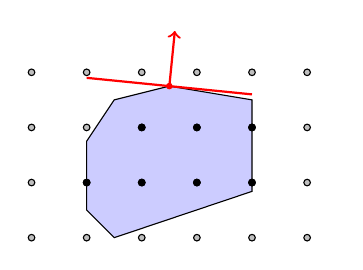
\begin{tikzpicture}[scale=.7]
				% styles
				\tikzstyle{polylp} += [draw,fill=blue!20]
				\tikzstyle{obj} += [draw=red,thick]
				
				% bounding box
				\draw[white] (0,1) rectangle (5.5,4.8);
				
				% polytope (first slide)
				\path[polylp] (1.0,2.75) -- (1.5,3.5) -- (2.5,3.75) -- (4,3.5)
				-- (4.0,1.84) -- (1.5,1.0) -- (1.0,1.5) -- cycle;
				
				% grid points
				\foreach \x in {0,...,5}
				\foreach \y in {1,...,4}
				{
					\draw[fill=black!25] (\x,\y) circle (0.06);
				}
				
				% integer points
				\foreach \x in {2,3,4}
				\foreach \y in {2,3}
				{
					\draw[fill=black] (\x,\y) circle (0.06);
				}
				\draw[fill=black] (1,2) circle (0.06);
				
				% objective
				\path[obj] (1,3.9) -- (4.0,3.6);
				\path[obj,->] (2.5,3.75) -- (2.6,4.75);
				\draw[fill=red,draw=none] (2.5,3.75) circle (0.06);
			\end{tikzpicture}
		\end{column}
	\end{columns}
	\vfill
	
	\vspace{0.5em}
	Useful properties of the LP relaxation:
	\begin{itemize}
		\item The constraint set $\sum_{j} a_{ij} x_j \geq b_i$ forms a convex polytope, and the optimal solution can be found in \textbf{polynomial time} (so efficiently)
		\item Its solution is \inference{informative} for the (M)ILP solution
	\end{itemize}
\end{frame}

\begin{frame}{\textit{Mixed} Integer Linear Programming (M)ILP: \inference{inference}}
	LP relaxation:
	\begin{columns}[T,totalwidth=\textwidth]
		\begin{column}{0.54\textwidth}
			{\footnotesize
				\[
				\begin{aligned}
					& \text{minimize}   && \sum_j c_j\, x_j \\
					& \text{subject to} && \sum_{j} a_{ij}\, x_j \ge b_i \quad \text{for } i=1,\ldots,m \\
					&                   && x_j \in \mathbb{R} \cap [\ell_j,u_j] \quad \text{(possibly $\pm\infty$)}
				\end{aligned}
				\]
			}
		\end{column}
		\begin{column}{0.46\textwidth}
			\centering
			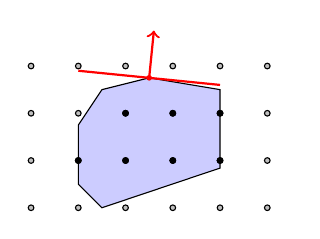
\begin{tikzpicture}[scale=.6]
				% styles
				\tikzstyle{polylp} += [draw,fill=blue!20]
				\tikzstyle{obj} += [draw=red,thick]
				
				% bounding box
				\draw[white] (0,1) rectangle (5.5,4.8);
				
				% polytope (first slide)
				\path[polylp] (1.0,2.75) -- (1.5,3.5) -- (2.5,3.75) -- (4,3.5)
				-- (4.0,1.84) -- (1.5,1.0) -- (1.0,1.5) -- cycle;
				
				% grid points
				\foreach \x in {0,...,5}
				\foreach \y in {1,...,4}
				{
					\draw[fill=black!25] (\x,\y) circle (0.06);
				}
				
				% integer points
				\foreach \x in {2,3,4}
				\foreach \y in {2,3}
				{
					\draw[fill=black] (\x,\y) circle (0.06);
				}
				\draw[fill=black] (1,2) circle (0.06);
				
				% objective
				\path[obj] (1,3.9) -- (4.0,3.6);
				\path[obj,->] (2.5,3.75) -- (2.6,4.75);
				\draw[fill=red,draw=none] (2.5,3.75) circle (0.06);
			\end{tikzpicture}
		\end{column}
	\end{columns}
	\vfill
	
	\vspace{0.5em}
	\inference{Inference} with the LP relaxation:
	\begin{itemize}
		\item If the LP relaxation has \textbf{no solution}, the MIP problem has no solution either
		\item If the \textbf{optimal solution} to the LP relaxation is integral, then it is an optimal solution to the ILP problem (similarly for a mixed problem)
	\end{itemize}
	\vfill
	
	What if it has a solution that is not fully integral?
\end{frame}


\begin{frame}{\textit{Mixed} Integer Linear Programming (M)ILP: \inference{inference 2}}
	
	What if the LP relaxation solution is not fully integral?
	\vfill
	
	{\footnotesize
	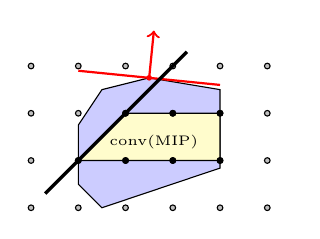
\begin{tikzpicture}[scale=.6]
		% styles
		\tikzstyle{polylp} += [draw,fill=blue!20]
		\tikzstyle{polyconv} += [draw,fill=yellow!20]
		\tikzstyle{obj} += [draw=red,thick]
		\tikzstyle{txt} += [font=\tiny]
		\tikzstyle{cut} += [draw=black,very thick]
		
		% bounding box
		\draw[white] (0,1) rectangle (5.5,4.8);
		
		% polytope (first slide)
		\path[polylp] (1.0,2.75) -- (1.5,3.5) -- (2.5,3.75) -- (4,3.5)
		-- (4.0,1.84) -- (1.5,1.0) -- (1.0,1.5) -- cycle;
		
		\visible<2->{
			% conv hull, 2nd slide
			\path[polyconv] (1,2) -- (2,3) -- (4,3) -- (4,2) -- cycle;
			\draw (2.6,2.4) node[txt]{conv(MIP)};
		}
		
		% grid points
		\foreach \x in {0,...,5}
		\foreach \y in {1,...,4}
		{
			\draw[fill=black!25] (\x,\y) circle (0.06);
		}
		
		% integer points
		\foreach \x in {2,3,4}
		\foreach \y in {2,3}
		{
			\draw[fill=black] (\x,\y) circle (0.06);
		}
		\draw[fill=black] (1,2) circle (0.06);
		
		% objective
		\path[obj] (1,3.9) -- (4.0,3.6);
		\path[obj,->] (2.5,3.75) -- (2.6,4.75);
		\draw[fill=red,draw=none] (2.5,3.75) circle (0.06);
		
		% cut
		\visible<3>{
			\path[cut] (0.3,1.3) -- (3.3,4.3);
		}  
	\end{tikzpicture}
	}
	\vfill
	
	\only<2>{
	Observe: there exists a set of constraints such that an LP relaxed solution is the MILP solution: the convex hull of the integer feasible solutions.
	\vfill
	
	\begin{itemize}
		\item But the linear description is not known...
		\item and it has a large number of constraints.
	\end{itemize}
	}
	\visible<3>{
	\inference{Inference method 2: cutting planes}
	
	Infering additional constraints (cuts) that cut away the LP solution and bring us close to the MILP solution (without cutting integral solutions away).
	}
\end{frame}

\begin{frame}{\textit{Mixed} Integer Linear Programming (M)ILP: \inference{inference 2}}
	
	\begin{columns}[T,totalwidth=\textwidth]
		\begin{column}{0.64\textwidth}
			Many cutting plane generation algorithms exist:
			\begin{itemize}
				\item Gomory cuts (for pure integer programs, guaranteed to converge)
				\item Mixed Integer Rounding (MIR) cuts
				\item Cover cuts
				\item Lift-and-project cuts
				\item ...
			\end{itemize}
		\end{column}
		\begin{column}{0.36\textwidth}
			\vspace{1em}
			{\footnotesize
				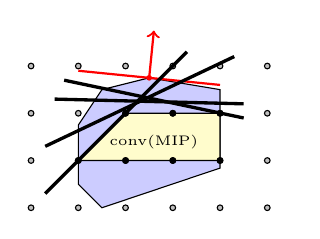
\begin{tikzpicture}[scale=.6]
					% styles
					\tikzstyle{polylp} += [draw,fill=blue!20]
					\tikzstyle{polyconv} += [draw,fill=yellow!20]
					\tikzstyle{obj} += [draw=red,thick]
					\tikzstyle{txt} += [font=\tiny]
					\tikzstyle{cut} += [draw=black,very thick]
					
					% bounding box
					\draw[white] (0,1) rectangle (5.5,4.8);
					
					% polytope (first slide)
					\path[polylp] (1.0,2.75) -- (1.5,3.5) -- (2.5,3.75) -- (4,3.5)
					-- (4.0,1.84) -- (1.5,1.0) -- (1.0,1.5) -- cycle;
					
					\visible<1>{
						% conv hull, 2nd slide
						\path[polyconv] (1,2) -- (2,3) -- (4,3) -- (4,2) -- cycle;
						\draw (2.6,2.4) node[txt]{conv(MIP)};
					}
					
					% grid points
					\foreach \x in {0,...,5}
					\foreach \y in {1,...,4}
					{
						\draw[fill=black!25] (\x,\y) circle (0.06);
					}
					
					% integer points
					\foreach \x in {2,3,4}
					\foreach \y in {2,3}
					{
						\draw[fill=black] (\x,\y) circle (0.06);
					}
					\draw[fill=black] (1,2) circle (0.06);
					
					% objective
					\path[obj] (1,3.9) -- (4.0,3.6);
					\path[obj,->] (2.5,3.75) -- (2.6,4.75);
					\draw[fill=red,draw=none] (2.5,3.75) circle (0.06);
					
					% cut
					\visible<1>{
						\path[cut] (0.3,1.3) -- (3.3,4.3);
						\path[cut] (0.3,2.3) -- (4.3,4.2);
						\path[cut] (0.5,3.3) -- (4.5,3.2);
						\path[cut] (0.7,3.7) -- (4.5,2.9);
					}  
				\end{tikzpicture}
			}
		\end{column}
	\end{columns}
	\vspace{1em}
	\vfill
	
	Cutting plane generation is a powerful \inference{inference method}, but in practice:
	\begin{itemize}
		\item Slow to converge
		\item Smart cut selection as well as aging is important
		\item Best combined with \search{branch-and-bound}: branch-and-cut
	\end{itemize}
	
\end{frame}


\begin{frame}{Branch-and-cut}
	Limited cutting plane generation at root and nodes of a branch-and-bound tree.
	\vfill
	
	\textbf{LP-based branch-and-bound:}\\
	Systematic reduction of $UB-LB$ by divide-and-conquer. %\cite{LandDoig1960,Dakin1965}
	\bigskip
	
	\begin{minipage}[t]{.45\textwidth}
		\centering
		\textbf{Branch-and-bound tree}
		
		\vspace*{3em}
		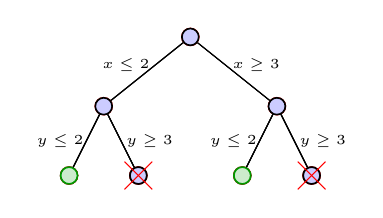
\begin{tikzpicture}[auto,scale=0.88]	
  \tikzstyle{bbnode}=[circle,draw=black,fill=blue!20,semithick,inner sep=.5ex]
  \tikzstyle{var}=[rectangle,node distance=3ex];
  \tikzstyle{txt} += [font=\tiny]
  
  \alt<2-4>
  { \node (root) at (2.25,4) [bbnode,red,fill=red!20] {};}
  { \node (root) at (2.25,4) [bbnode] {}; } 
  
  
  \visible<4->{
    \alt<5-7>
    { \node (fork1) at (1,3) [bbnode,red,fill=red!20]{} edge (root);}
    { \node (fork1) at (1,3) [bbnode]{} edge (root);}
    
    \alt<15-17>
    { \node (fork2) at (3.5,3) [bbnode,red,fill=red!20]{} edge (root); }
    { \node (fork2) at (3.5,3) [bbnode]{} edge (root); }
    
    \draw (1.32,3.6) node[txt]{$x \leq 2$};
    \draw (3.2,3.6) node[txt]{$x \geq 3$};
  }
  
  \visible<7->{
    \temporal<8-9>
    { \node (leaf1) at (.5,2) [bbnode]{} edge (fork1);}
    { \node (leaf1) at (.5,2) [bbnode,red,fill=red!20]{} edge (fork1);}
    { \node (leaf1) at (.5,2) [bbnode,green!60!black,fill=green!60!black!20]{} edge (fork1);}
    
    \temporal<12-13>
    { \node (leaf2) at (1.5,2) [bbnode]{} edge (fork1);}  
    { \node (leaf2) at (1.5,2) [bbnode,red,fill=red!20]{} edge (fork1);}  
    { \node (leaf2) at (1.5,2) [bbnode]{} edge (fork1);
      \path[draw=red] (1.3,2.2) -- (1.7,1.8);
      \path[draw=red] (1.3,1.8) -- (1.7,2.2);
    }

	\draw (0.37,2.5) node[txt]{$y \leq 2$};
	\draw (1.66,2.5) node[txt]{$y \geq 3$};
  }

  \visible<17->{
    \temporal<18-19>
    { \node (leaf3) at (3,2) [bbnode]{} edge (fork2);}
    { \node (leaf3) at (3,2) [bbnode,red,fill=red!20]{} edge (fork2);}
    { \node (leaf3) at (3,2) [bbnode,green!60!black,fill=green!60!black!20]{} edge (fork2);}
    
    \temporal<22-23>
    { \node (leaf4) at (4,2) [bbnode]{} edge (fork2);}  
    { \node (leaf4) at (4,2) [bbnode,red,fill=red!20]{} edge (fork2);}  
    { \node (leaf4) at (4,2) [bbnode]{} edge (fork2);
      \path[draw=red] (3.8,2.2) -- (4.2,1.8);
      \path[draw=red] (3.8,1.8) -- (4.2,2.2);
    }

	\draw (2.87,2.5) node[txt]{$y \leq 2$};
	\draw (4.16,2.5) node[txt]{$y \geq 3$};
  }
\end{tikzpicture}
	\end{minipage}
	\hfill
	\begin{minipage}[t]{.45\textwidth}
		\centering
		\textbf{Solution space}
		\vspace*{-1em}
		
		\begin{center}
  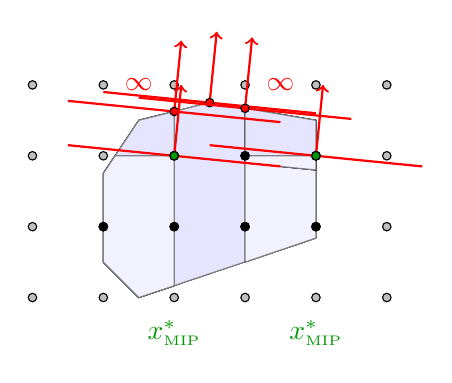
\begin{tikzpicture}[scale=.9]
    \tikzstyle{new} += [draw,fill=blue!20]
    \tikzstyle{old} += [draw=black!50,fill=blue!10]
    \tikzstyle{cutoff} += [draw=black!50,fill=blue!5]

    % --------BOUNDING-BOX--------%
    \draw[white] (0,1) rectangle (5.5,4.8);

    % ----------POLYTOP-----------%
    \visible<1-3>{
      \path[new] (1.0,2.75) -- (1.5,3.5)-- (2.5,3.75) -- (4,3.5) -- (4.0,1.84) -- (1.5,1.0) --(1.0,1.5)--cycle;
    }

    % ----------BranchBound----------%
    \visible<4>{
      \path[old] (1.0,2.75) -- (1.5,3.5)-- (2.5,3.75) -- (4,3.5) -- (4.0,1.84) -- (1.5,1.0) --(1.0,1.5)--cycle;
      \path[new] (3.0,3.67) -- (4,3.5) -- (4.0,1.84) -- (3.0,1.5) -- cycle;
    }
    \visible<4-6>{
      \path[new] (1.0,2.75) -- (1.5,3.5)-- (2.0,3.625) -- (2.0,1.166) -- (1.5,1.0) -- (1.0,1.5) -- cycle;
    }
    \visible<5-11>{
      \path[old] (3.0,3.67) -- (4,3.5) -- (4.0,1.84) -- (3.0,1.5) -- cycle;
    }
    \visible<7>{
      \path[old] (1.0,2.75) -- (1.5,3.5)-- (2.0,3.625) -- (2.0,1.166) -- (1.5,1.0) -- (1.0,1.5) -- cycle;
    }
    \visible<7-10>{
      \path[new] (1.0,2.75) -- (1.166,3.0) -- (2,3) --(2.0,1.166) -- (1.5,1.0) -- (1.0,1.5) -- cycle;
    }
    \visible<11>{
      \path[cutoff] (1.0,2.75) -- (1.166,3.0) -- (2,3) --(2.0,1.166) -- (1.5,1.0) -- (1.0,1.5) -- cycle;
      \path[cutoff] (3.0,2.9) -- (4,2.8) -- (4.0,1.84) -- (3.0,1.5) -- cycle;
    }
    \visible<15-16>{
      \path[new] (3.0,3.67) -- (4,3.5) -- (4.0,2.8) -- (3.0,2.9) -- cycle;
    }
    \visible<12-14,17>{
      \path[old] (3.0,3.67) -- (4,3.5) -- (4.0,2.8) -- (3.0,2.9) -- cycle;
    }
    \visible<17-20>{
      \path[new] (3.0,3) -- (4,3) -- (4.0,2.8) -- (3.0,2.9) -- cycle;
    }
    \visible<21>{
      \path[cutoff] (3.0,3) -- (4,3) -- (4.0,2.8) -- (3.0,2.9) -- cycle;
    }
    
    % ----------GITTER-------------%
    \foreach \x in {0,...,5}
    \foreach \y in {1,...,4}
    {
      \draw[fill=black!25] (\x,\y) circle (0.06);
    }
    % ----------GANZ----------------%
    \foreach \x in {2,3,4}
    \foreach \y in {2,3}
    {
      \draw[fill=black] (\x,\y) circle (0.06);
    }
    \draw[fill=black] (1,2) circle (0.06);


    % ----------OBJECTIVE-----------%
    \visible<3-4>{
      \path[draw=red, thick] (1,3.9) -- (4.0,3.6);
      \path[draw=red,thick,->] (2.5,3.75) -- (2.6,4.75);
      \draw[fill=red] (2.5,3.75) circle (0.06);
    }
    \visible<6-7>{
      \path[draw=red, thick] (0.5,3.775) -- (3.5,3.475);
      \path[draw=red,thick,->] (2.0,3.625) -- (2.1,4.625);
      \draw[fill=red] (2.0,3.625) circle (0.06);
    }
    \visible<9-11>{
      \path[draw=red, thick] (0.5,3.15) -- (3.5,2.85);
      \path[draw=red,thick,->] (2.0,3.0) -- (2.1,4.0);
    }
    \visible<9>{
      \draw [fill=red] (2.0,3.0) circle (0.06);
    }
    \visible<10-19>{
      \draw [fill=green!60!black] (2.0,3.0) circle (0.06);
    }
    \visible<10-19>{
      \node (a) at (2,.5) []{\textcolor{green!60!black}{$x_{\tiny\mbox{MIP}}^{*}$}};
    }
    \visible<12>{
      \node (a) at (1.5,4) []{\textcolor{blue!50}{$\varnothing$}};
    }
    \visible<13-14>{
      \node (a) at (1.5,4) []{\textcolor{red}{$\infty$}};
    }
    \visible<22>{
      \node (a) at (3.5,4) []{\textcolor{blue!50}{$\varnothing$}};
    }
    \visible<23-24>{
      \node (a) at (3.5,4) []{\textcolor{red}{$\infty$}};
    }
    \visible<16-17>{
      \path[draw=red, thick] (1.5,3.82) -- (4.5,3.52);
      \path[draw=red,thick,->] (3,3.67) -- (3.1,4.67);
      \draw [fill=red] (3,3.67) circle (0.06);
    }
    \visible<19-21>{
      \path[draw=red, thick] (2.5,3.15) -- (5.5,2.85);
      \path[draw=red,thick,->] (4,3) -- (4.1,4.0);
      \draw[fill=red] (4,3) circle (0.06);
    }
    \visible<20->{
      \draw[fill=green!60!black] (4,3) circle (0.06);
    }
    \visible<20->{
      \node (a) at (4,.5) []{\textcolor{green!60!black}{$x_{\tiny\mbox{MIP}}^{*}$}};
   }
  \end{tikzpicture}
\end{center}

	\end{minipage}
	\vfill
	
	\only<3,6,16>{\footnotesize (For illustration purposes, no cutting planes are generated)}
\end{frame}



\begin{frame}{Efficient MILP solvers}
	
	Many additional techniques:
	\begin{itemize}
		\item incremental LP computation: each LP call is \textit{warmstarted} from previous LP solution
		\item pre-solving: more effort in the root node
		\item primal heuristics (e.g. local search)
		\item branching heuristics and node selection
		\item cut generation, selection, and \textit{management}
		\item symmetry detection and handling
		\item parallelization
		%\item restarts
		%\item reduced cost fixing
		\item \ldots
	\end{itemize}
\end{frame}


\iffalse
\begin{frame}{IP Solving}
  \begin{itemize}
    \item Guarantee: exact, given enough time. \vfill
    \item Mainly black-box: limited ways to guide the solving. \vfill
    \item It scales well to thousands of variables.
      \vfill
    \item \alert{Any combinatorial problem can be encoded into IP.} \\
      (but it might require an exponential number of constraints) \vfill
    \item Advantages of ILP solving:
      \begin{itemize}
        \item Provides both a lower bound and an upper bound on the
          objective value of optimal solutions, if stopped early.
        \item Strong guidance by objective function (through LP solving)
        \item Naturally extends to MIP solving.
        \item \dots
      \end{itemize} \vfill
    \item Central method of operations research (OR), \\ applied in
      production planning, linear assignment problems, \dots
  \end{itemize}
\end{frame}
\fi

\subsection*{Transformation: linearize}
\begin{frame}{Overview}
\begin{tikzpicture}[scale=0.7, every node/.style={transform shape}, node distance=0.5cm]

\waterfall[linearize]
\end{tikzpicture}
\end{frame}

\begin{frame}{Linearisation of flat models}
	Assume all unsupported global constraints are decomposed, and all constraints are flattened.
	\vfill
	
	We've covered how $\sum_{j} a_{ij} x_j \leq b_i$, $\sum_{j} a_{ij} x_j = b_i$, and $\sum_{j} a_{ij} x_j > b_i$ can be rewritten to $\sum_{j} a_{ij} x_j \geq b$ form. Same for disjunctions $x_1 \vee \neg x_2 \vee x_3$.
	\vfill
	
	What about \textbf{reification} $d \rightarrow \text{Expr}$ (with $d$ a Boolean decision variable)?
\end{frame}


\begin{frame}{Linearisation of implications}
	Let's recap the truth table of $d \rightarrow e$:
	
	{\small \[
	\begin{array}{c|c||c}
		d & e & d \rightarrow e \\
		\hline
		T & T & T \\
		T & F & F \\
		F & T & T \\
		F & F & T
	\end{array}
	\] }
	\vfill
	
	If $d$ and $e$ are Boolean (0/1) variables: 
	\begin{itemize}
		\item $d \rightarrow e ~\Leftrightarrow~ (\neg d) \lor e ~\Leftrightarrow~ (1-d) + e \geq 1 ~\Leftrightarrow~ e \geq d$.
		\item Indeed, in case $d=1$ we have $e \geq 1$ which means $e$ must be true; \\
		in case $d=0$ we want $e$ to be unconstrained, and indeed we have $e \geq 0$ which is always true because lower-bound $lb(e) = 0$.
	\end{itemize}
\end{frame}

\begin{frame}{Linearisation of implications: Big-M}
	Consider $d \rightarrow x \geq 3$ with $0 \leq x \leq 10$.\\
	
	\begin{itemize}
		\item In case $d=1$: we want $x \geq 3$ to be true. Let's rewrite the latter as $x - 3 \geq 0$. So in case $d=1$ we could write $x - 3 \geq (1-d)$.
		\pause
		\item In case $d=0$: we want $x - 3$ to be unconstrained. Is there a constant $M$ such that $x - 3 \geq M$ would always be true? YES! its $M = lb(x - 3) = lb(x) - 3$.
		\pause
		\item So we can combine both cases in the linear inequality $x - 3 \geq M\cdot(1-d)$ with $M = lb(x-3)$ (or any value below that). It enforces the desired relation when $d=1$ and it is unconstrained when $d=0$.
	\end{itemize}
	\vfill
	\pause
	
	The above technique is called a Big-M formulation of a logical constraint. It is used to model all sorts of implications and logical equivalences. 
	\vfill
	
	For example: $d \rightarrow (x=3) ~\Leftrightarrow~ (d \rightarrow x \geq 3) \land (d \rightarrow x \leq 3)$ \\
	\qquad \qquad \qquad \qquad \qquad \qquad $~\Leftrightarrow~ (x - 3 \geq M_1\cdot (1-d)) \land (x - 3 \leq M_2\cdot (1-d))$.
\end{frame}


\begin{frame}{Linearisation of implications: more Big-M}
	Consider $x \neq 3$. This is not easily rewritable in inequalities.
	\vfill
	
	\begin{itemize}
		\item It is logically equivalent to splitting into the disjunctive cases $(x > 3) \lor (x < 3)$.
		\item For integers: $(x \geq 4) \lor (x \leq 2)$, then $(d \lor e) \land (d \rightarrow x \geq 4) \land (e \rightarrow x \leq 2)$.
		\item Big-M reformulation: $x - 4 \geq M_1\cdot (1-d)$ and $x - 2 \leq M_2\cdot (1-e)$.
		\item Together: $(d + e \geq 1) \land (x - 4 \geq M_1\cdot (1-d)) \land (x - 2 \leq M_2\cdot (1-e))$
	\end{itemize}
	\vfill
	\pause
		
	But we can go one step further: we know that $(x \geq 4)$ and $(x \leq 2)$ can never happen at the same time, and hence neither can $d$ and $e$. Combined with $d + e \geq 1$ we have $d + e = 1$ and hence $d = 1-e$, allowing us to eliminate $e$:
	\begin{itemize}
		\item we \textbf{only need two constraints and one auxiliary variable} to linearize $x \neq 3$: $(x - 4 \geq M_1\cdot (1-d)) \land (x - 2 \leq M_2\cdot d)$.
	\end{itemize}
	\pause
	
	The same reasoning can be applied to $x \neq y$ and $\sum_j a_j \cdot x_j \neq b$.
\end{frame}

\begin{frame}{Linearization of implications: general Big-M}
	For a general linear \textit{indicator} constraint:
	\vspace{-0.5em}
	\[
	d = 1 \rightarrow \sum_{j} a_{ij}x_j \leq b 
	\quad\Leftrightarrow\quad \sum_{j} a_{ij}x_j - b \leq M(1-d)
	\]
	\vspace{-0.5em}
	
	We want a \textbf{small} 
	$M = \max \{ \sum_{j} a_{ij}x_j - b : \text{ feasible } x \}$
	
	
	Why?
	\begin{itemize}
		\item Big M's can lead to poor LP relaxations
		\item Really big M's can lead to numeric instability\\
		Some ILP solvers accept indicator constraints, and for really big M's may defer their linearisation until it is smaller later in the branch-and-bound tree.
	\end{itemize}
	\pause
	
	Computing $M$ by knowing what is 'feasible':
	
	\begin{itemize}
		\item The base case is the maximum over the box relaxation: \\
		$M = \sum_{j : a_{ij} < 0} a_{ij} \cdot lb(x_j) + \sum_{j : a_{ij} > 0} a_{ij} \cdot ub(x_j) - b$
		
		\item More advanced approaches can use additional information, such as subsets of Boolean $x$ that are at-most-1 (take their max instead of sum) or other constraints that lead to a smaller M.
	\end{itemize}
	
\end{frame}

\begin{frame}{Linearly encoding all values of a domain}
	Given an integer variable $1 \leq x \leq 10$.
	\vfill
	
	To encode one of its values as $d_3 \leftrightarrow (x = 3)$ we would need $4$ constraints: two for $d_3 \rightarrow(x=3)$ and two for $(\neg d_3) \rightarrow x \neq 3$ {\small(verify this yourself with the previous slide)}.
	% for d -> (x=3) as before
	% for d -> (x!=3) substitute d -> (x-3>M1(1-e) & x-3<M2(e)) and split
	\vfill 
	\pause
	
	However, if we know we are going to encode \textbf{each} value of $x$, e.g.
	$d_1 \leftrightarrow (x = 1) \land ... \land d_{10} \leftrightarrow (x = 10)$ then there is a much simpler encoding:
	\begin{align*}
		d_1 + d_2 + ... + d_{10} = 1 \\
		1\cdot d_1 + 2\cdot d_2 + ... + 10\cdot d_{10} = x 
	\end{align*}
	So just 2 constraints to encode all 10 Booleans...
	\vfill
	\pause
	
	You can go even further and \textit{eliminate} all occurrences of $x$ using the last equality...
\end{frame}

\begin{frame}{Linearising \cons{AllDifferent}{}}
	Which of the following two $\cons{AllDifferent}{x_1, x_2, \ldots, x_n}$ decompositions do you think is best for an ILP solver?
	\vfill
	
	{\small
	\begin{align*}
		&x_i \neq x_j &&\text{ for } i=1,\ldots,n \quad \text{for } j=i+1,\ldots,n
	\end{align*}
	}
	\vfill
	
	or:
	{\small
	\begin{align*}
		&\sum_{v \in D(x_i)} v\cdot d_{iv} = x_i &&\text{ for } i=1,\ldots,n \\
		&\sum_{v \in D(x_i)} d_{iv} = 1 &&\text{ for } i=1,\ldots,n \\
		&\sum_{i=1..n} d_{iv} \leq 1 &&\text{ for } v=min_i(D(x_i)),\ldots,max_i(D(x_i))
	\end{align*}
	}
	\vfill
	\pause
	
	The latter is the \textbf{linear (flow-graph) decomposition} from lecture~3. Creating the 'domain value' $d_{iv}$ auxiliary variables per integer variable allows for a tighter LP relaxation than when creating Big-M-ed 'not equals' auxiliary variables per pair of integer variables.
\end{frame}

\begin{frame}{Linearising global constraints}
	Creating 'domain value' $d_{iv}$ auxiliary variables per integer variable  $x_i$ is a good \textbf{pattern} for many global constraints that do domain-consistent reasoning!
	\vfill
	
	Other examples, let $X = [x_1, x_2, \ldots, x_n]$ an array of integer decision variables:
	\begin{itemize}
		\item \cons{CountEq}{$X, v, res$}: $(res = \sum_i d_{iv})$
		\item \cons{GlobalCardinalityCount}{$X, Vs, Res$}: $\forall v \in Vs: (Res_v = \sum_i d_{iv})$
		\item \cons{NValueEq}{$X, res$}: $(res = \sum_v b_v) \land \left(\forall v \in Vals: (b_v = (\sum_i d_{iv} \geq 1))\right)$
		\item \cons{ElementEq}{$Arr, x_i, res$}: $(res = \sum_v Arr_v\cdot d_{iv})$
		%\item \cons{Table}{$X, T$}: Let $e_r$ be a Boolean variable for each row in $T$, then $(\forall i: (X_i = \sum_r T_{ri} \cdot e_r)) \land (\sum_r e_r = 1)$
		\item Also for \cons{Table}{$X, T$}, \cons{MaxEq}{$X, res$}, \cons{Prod}{$x_i, x_j, res$} and more.
	\end{itemize}
	\vfill
	\pause
	
	In fact, ILP modellers typically only use integer variables for \textit{relaxable} quantities (where a fractional $x_i = 3.6$ makes sense, like quantity, volume, flow),\\
	and otherwise directly model over Boolean variables for the discrete options $d_{iv}$.
\end{frame}

\iffalse
\begin{frame}{ILP solvers}
  \begin{itemize}
    \item \href{https://www.scipopt.org}{SCIP} (open-source)
    \item \href{https://github.com/coin-or/Cbc}{Cbc} (open-source)
    \item \href{https://highs.dev}{HiGHS} (open-source)
    \item \href{https://www.gurobi.com}{Gurobi Optimizer} (commercial:
      requires a license)
    \item \href{https://www.ibm.com/products/ilog-cplex-optimization-studio/cplex-optimizer}{IBM CPLEX Optimizer} (commercial: requires a license)
    \item \href{https://www.fico.com/en/products/fico-xpress-optimization}{FICO
        Xpress Solver} (commercial: requires a license)
  \end{itemize}
\end{frame}
\fi


\subsection*{Pseudo-Boolean (PB) Optimization}
% OVERVIEW: PB solver highlight
\begin{frame}{Overview}
\begin{tikzpicture}[scale=0.7, every node/.style={transform shape}, node distance=0.5cm]

\waterfall[pb2]
\end{tikzpicture}
\end{frame}


\begin{frame}{Pseudo-Boolean (PB) Solving}
  Only accepts \textbf{Pseudo-Boolean Constraints}: $\sum_{i=1}^n a_i x_i \leq b$, where $a_i, b$ are integer constants and $x_i$ are Boolean decision variables.
  \vfill
  
  Extends SAT by allowing linear inequalities over Boolean variables \\
  (equivalently: ILP restricted to 0/1 variables).
  \vfill
  \pause
  
  Two possible solving techniques:
  \begin{itemize}
  	\item Eagerly encode into SAT (see next part)
  	\item Develop a SAT-like solver with pseudo-boolean propagation and pseudo-boolean conflict analysis (not covered in lecture)\\
  	  Example such solvers: RoundingSAT, Exact
  \end{itemize}
  \vfill
  
  Pseudo-Boolean \textbf{Optimisation} (PBO): optimising a linear objective over Boolean variables.
\end{frame}


\subsection*{Transformation: int to bool}
\begin{frame}{Overview}
\begin{tikzpicture}[scale=0.7, every node/.style={transform shape}, node distance=0.5cm]

\waterfall[int2bool]
\end{tikzpicture}
\end{frame}


\begin{frame}{Encoding into (pseudo)Boolean constraints}
  \structured{Challenges:}
  \begin{itemize}
    \item How to encode an integer variable into a collection of Boolean
      variables?
    \item How to encode a constraint on integer variables into (a
      collection of) constraints on Boolean variables?
  \end{itemize}
  \vfill

  \structured{Considerations:}
  \begin{itemize}
    \item We want few variables.
    \item We want few constraints, or short constraints.
    \item We want strong propagation.
  \end{itemize}
  \vfill%

  As usual, there are many possibilities, which make different trade-offs.
\end{frame}

\begin{frame}{Encoding an Integer Variable}
  Well-known encodings, described on the next slides: \vfill
  \begin{itemize}
    \item \defined{Direct (or value or sparse or one-hot) encoding}: \\
      a Boolean 'equality' variable for each value in the domain. \vfill
    \item \defined{Order encoding}: \\
      a Boolean 'inequality' variable for each value in the domain. \vfill
    \item \defined{Log (or bit or binary) encoding}: \\
      a Boolean variable for each bit in the base-2 representation of
      the largest domain value.
  \end{itemize}
\end{frame}

\begin{frame}{Encodings: example with overview}
	
	Encodings for $x \in \{0,1,2,3\}$:
	
	\centering
	\begin{table}[h!]
		\small
		\centering
		\renewcommand{\arraystretch}{1.2}
		\begin{tabular}{c|cccc|ccc|cc}
			& \multicolumn{4}{c|}{Direct encoding} & \multicolumn{3}{c|}{Order encoding} & \multicolumn{2}{c}{Log encoding} \\ 
			$x$ & $b_{[x=0]}$ & $b_{[x=1]}$ & $b_{[x=2]}$ & $b_{[x=3]}$ & $b_{[x \ge 1]}$ & $b_{[x \ge 2]}$ & $b_{[x \ge 3]}$ & $b_{\text{bit}^1(x)}$ & $b_{\text{bit}^0(x)}$ \\ \hline
			0 & 1 & 0 & 0 & 0 & 0 & 0 & 0 & 0 & 0 \\
			1 & 0 & 1 & 0 & 0 & 1 & 0 & 0 & 0 & 1 \\
			2 & 0 & 0 & 1 & 0 & 1 & 1 & 0 & 1 & 0 \\
			3 & 0 & 0 & 0 & 1 & 1 & 1 & 1 & 1 & 1 \\
		\end{tabular}
	\end{table}
\end{frame}

\begin{frame}{\defined{Direct} Encoding of an Integer Variable}
  Consider an integer variable $x$ with domain $0..n$: \vfill
  \begin{itemize}
    \item Create a Boolean variable $b_{[x=k]}$ for all $k \in \{0..n\}$
      \vfill
    \item The variable $b_{[x=k]}$ is \textbf{true} if and only if
      $x = k$ holds \vfill
    \item Consistency constraint: \vfill
      \begin{itemize}
          \item Variable $x$ has exactly one value from domain: $\sum_{k=0}^n b_{[x=k]} = 1$
      \end{itemize} \vfill
    \item Example encodings of simple constraints:
      \begin{itemize}
        \item The constraint $x \neq k$ is encoded as $\lnot b_{[x=k]}$
          \vfill
        \item The constraint $x < k$ is encoded as
          $\bigwedge_{j \in \{k..n\}} \lnot b_{[x=j]}$
          \vfill
        \item In any constraint, can replace $x$ by $\sum_k k \cdot b_{[x=k]}$
      \end{itemize}
  \end{itemize}
\end{frame}

\begin{frame}{\defined{Order} Encoding of an Integer Variable}
  Consider an integer variable $x$ with domain $0..n$: \vfill
  \begin{itemize}
    \item Create a Boolean variable $b_{[x \geq k]}$ for all $k \in \{1..n\}$. \vfill
    \item The variable $b_{[x \geq k]}$ is \textbf{true} if and only if
      $x \geq k$ holds. \vfill
    \item Consistency constraint: \vfill
	  \begin{itemize}
        \item Monotone ordering: $\displaystyle\bigwedge_{k \in 1..(n-1)} \left(b_{[x \geq k+1]} \rightarrow b_{[x \geq k]} \right)$
      \end{itemize} \vfill
    \item Example encodings of simple constraints \\
	      (assume $b_{[x \geq 0]}$ returns True, $b_{[x \geq n+1]}$ returns False):
      \begin{itemize}
        \item The constraint $x = k$ is encoded as
          $b_{[x \geq k]} \land \lnot b_{[x \geq k+1]}$ \vfill
        \item The constraint $x \neq k$ is encoded as
          $\lnot b_{[x \geq k]} \lor b_{[x \geq k+1]}$ \vfill
        %\item The constraint $x < k$ is encoded as $\lnot b_{[x \geq k]}$.
        \item In any constraint, can replace $x$ by $\sum_k b_{[x \geq k]}$
      \end{itemize}
  \end{itemize}
\end{frame}

\begin{frame}{\defined{Log} Encoding of an Integer Variable}
  Consider an integer variable $x$ with domain $0..n$ (so $n+1$ values): \vfill
  \begin{itemize}
    \item Encode the value of $x$ in binary, using just $\lceil \log_2(n+1) \rceil$ Boolean variables. \vfill
    \item Let $b_i$ a Boolean variable representing the $i$-th bit in the binary encoding of $x$ (counting from the right, least significant bit). \vfill
    \item In any constraint, can replace $x$ by:
      \[
      x = \sum_{i=0}^{\lceil \log_2(n+1) \rceil - 1} b_i \cdot 2^i
      \]
      where $b_i \in \{0, 1\}$. \vfill
    \item Consistency constraint, in case $n+1$ is not a power of 2: 
      \begin{itemize}
        \item Upper bound of domain:  $\sum_{i=0}^{\lceil \log_2(n+1) \rceil - 1} b_i \cdot 2^i \leq n$
      \end{itemize}
      %
    %\item This encoding requires $\lceil \log_2(n+1) \rceil$ Boolean variables and a few additional constraints if $n+1$ is not a power of 2. \vfill
    %\item The constraint $x = k$ is encoded by setting the binary variables to match the binary representation of $k$. \vfill
    %\item The constraint $x \neq k$ is encoded by ensuring at least one bit in the binary representation of $x$ differs from that of $k$. \vfill
    %\item Constraints for inequalities like $x < k$ or $x > k$ can also be derived by comparing binary representations.
  \end{itemize}
\end{frame}


\subsection*{Boolean Satisfiability (SAT/MaxSAT)}
% OVERVIEW: SAT solver highlight
\begin{frame}{Overview}
\begin{tikzpicture}[scale=0.7, every node/.style={transform shape}, node distance=0.5cm]

\waterfall[sat2]
\end{tikzpicture}
\end{frame}

\begin{frame}{The SAT Problem}
	\begin{itemize}
		\item \defined{Decision variable} $x$: takes value \textbf{true} ($=1$) or \textbf{false} ($=0$)
		\vfill
		
		\item \defined{Literal} $\ell$: variable $x$ or its negation $\neg x$\\
		(which we will from now on write as $\overline{x}$ instead of $\neg x$)
		\vfill		
		
		\item \textbf{Primitive constraint} a \defined{clause} $C = \ell_1 \lor \cdots \lor \ell_{k}$ \quad disjunction of literals \\
		(considered as sets, so no repetitions and order irrelevant)
		\vfill
		
		\item \defined{Conjunctive normal form} (CNF) formula $F = C_1 \land \cdots \land C_m$ \quad conjunction of clauses         
	\end{itemize}
	\vfill
	
	\begin{block}{The SAT Problem}
		Given a CNF formula~$F$, is it satisfiable?
	\end{block}
	\vfill
	
	For instance, what about:
	%     \small
	\begin{gather*}
		( p \lor \overline{u} )
		\,\land\,
		( q \lor r )
		\,\land\,
		( \overline{r} \lor w )
		\,\land\,
		( u \lor x \lor y )
		\,\land\,
		\\ %%%
		( x \lor \overline{y} \lor z )
		\,\land\,
		( \overline{x} \lor z )
		\,\land\,
		( \overline{y} \lor \overline{z} )
		\,\land\,
		( \overline{x} \lor \overline{z} )
		\,\land\,
		( \overline{p} \lor \overline{u} )
	\end{gather*}
\end{frame}

% For highlighting in examples 
\newcommand<>{\alertred}[1]{{\color#2{red}#1}}
\newcommand<>{\alertblue}[1]{{\color#2[rgb]{0,0,0.7}#1}}
\newcommand<>{\alertgreen}[1]{{\color#2[rgb]{0,0.6,0}#1}}
\begin{frame}[t]{SAT propagation: unit propagation}
		
	\begin{block}{Unit Propagation}
		Clause $C$ \defined{unit propagates} $\ell$ under partial assignment $\rho$ if $\rho$ falsifies all literals in $C$ except $\ell$.
	\end{block}
	\vfill
	
	\textbf{Example:} Unit propagate for $\rho = \{ p \mapsto 0, q\mapsto 0 \}$ on
	\begin{equation*}%
		( 
		\alertred<2->{p} \lor 
		\alertgreen<3->{\overline{u}}
		)
		\,\land\, 
		( \alertred<2->{q}
		\lor
		\alertgreen<4->{r} 
		)
		\,\land\,
		(
		\alertred<4->{\overline{r}}
		\lor 
		\alertgreen<5->{w} 
		)
		\,\land\,
		( 
		\alertred<3->{u}
		\lor x \lor y )
		\,\land\,
		( x \lor \overline{y} \lor z )
		\,\land\,
		( \overline{x} \lor z )
		\,\land\,
		( \overline{y} \lor \overline{z} )
		\,\land\,
		( \overline{x} \lor \overline{z} )
		\,\land\,
		( 
		\alertgreen<2->{\overline{p}} 
		\lor
		\alertgreen<3->{\overline{u}}
		)
	\end{equation*}
	\vfill
	
	\begin{itemize}
		\item<3-> $p \lor \overline{u}$ propagates $u \mapsto 0$
		
		\item<4-> $q \lor r$ propagates $r \mapsto 1$
		
		\item<5-> Then $\overline{r} \lor w$ propagates $w \mapsto 1$
		
		\item<6-> No further unit propagations
	\end{itemize}
\end{frame}


% Custom colors
\definecolor{failpurple}{RGB}{204,121,167}
\usetikzlibrary{decorations.pathreplacing}

\begin{frame}{Conflict-Driven Clause Learning (CDCL)}
	\vspace{-1em}
	\quad CDCL combines \inference{unit propagation} and \search{search} with \inference{conflict analysis}.
	
	\vspace{-1.5em}
	\[
	( p \lor \overline{u} )
	\,\land\,
	( q \lor r )
	\,\land\,
	( \overline{r} \lor w )
	\,\land\,
	( u \lor x \lor y )
	\,\land\,
	( x \lor \overline{y} \lor z )
	\,\land\,
	( \overline{x} \lor z )
	\,\land\,
	( \overline{y} \lor \overline{z} )
	\,\land\,
	( \overline{x} \lor \overline{z} )
	\,\land\,
	( \overline{p} \lor \overline{u} )
	\]
	\pause
	
	\vspace{-1em}
	\begin{columns}
		\begin{column}{0.35\textwidth}
			\centering
			\begin{tikzpicture}[node distance=0.08cm]
				% styles
				\tikzstyle{base} = [draw, font=\scriptsize, minimum width=1.6cm]
				\tikzstyle{decis} += [base, draw=Orange]
				\tikzstyle{prop}  += [base, dashed, draw=LimeGreen]
				\tikzstyle{fail}  += [base]
				
				\visible<2->{
					\node[decis] (p) {$p \overset{\text{d}}{=} 0$};
				}
				\visible<3->{
					\node[below=of p, prop] (u) {$u \overset{p \lor \bar{u}}{=} 0$};
				}
				\visible<4->{
					\node[below=of u, decis] (q) {$q \overset{\text{d}}{=} 0$};
				}
				\visible<5->{
					\node[below=of q, prop] (r) {$r \overset{q \lor r}{=} 1$};
				}
				\visible<6->{
					\node[below=of r, prop] (w) {$w \overset{\bar{r} \lor w}{=} 1$};
				}
				\visible<7->{
					\node[below=of w, decis] (x) {$x \overset{\text{d}}{=} 0$};
				}
				\visible<8->{
					\node[below=of x, prop] (y) {$y \overset{u \lor x \lor y}{=} 1$};
				}
				\visible<9->{
					\node[below=of y, prop] (z) {$z \overset{x \lor \bar{y} \lor z}{=} 1$};
				}
				\visible<10->{
					\node[below=of z, fail] (bot) {$\overset{\bar{y} \lor \bar{z}}{\textcolor{failpurple}{\bot}}$};
				}
			\end{tikzpicture}
		\end{column}
		
		\begin{column}{0.6\textwidth}
			\textbf{\search{Search decision}}\\
			Free choice to assign value to variable\\
			Notation {$p \overset{\text{d}}{=} 0$}\\[0.5em]
			\pause
			
			\textbf{\inference{Unit propagation}}\\
			Forced choice to avoid falsifying clause\\
			Given $p=0$, clause $p \lor \bar{u}$ forces $u=0$\\
			Notation {$u \overset{p \lor \bar{u}}{=} 0$} ($p \lor \bar{u}$ is reason clause)\\[1em]
			\pause
			
			Always propagate if possible, otherwise decide\\
			Add to assignment \textit{trail}\\
			Continue until satisfying assignment or \textcolor{failpurple}{conflict}
		\end{column}
	\end{columns}
\end{frame}


\begin{frame}{CDCL, conflict analysis}
	\vspace{-1em}
	\quad CDCL combines \inference{unit propagation} and \search{search} with \inference{\textbf{conflict analysis}}.
	
	\vspace{-1.5em}
	\[
	( p \lor \overline{u} )
	\,\land\,
	( q \lor r )
	\,\land\,
	( \overline{r} \lor w )
	\,\land\,
	( u \lor x \lor y )
	\,\land\,
	( x \lor \overline{y} \lor z )
	\,\land\,
	( \overline{x} \lor z )
	\,\land\,
	( \overline{y} \lor \overline{z} )
	\,\land\,
	( \overline{x} \lor \overline{z} )
	\,\land\,
	( \overline{p} \lor \overline{u} )
	\]
	
	\vspace{-0.5em}
	\begin{columns}
		\begin{column}{0.35\textwidth}
			\centering
			\begin{tikzpicture}[node distance=0.08cm]
				% styles
				\tikzstyle{base} = [draw, font=\scriptsize, minimum width=1.6cm]
				\tikzstyle{decis} += [base, draw=Orange]
				\tikzstyle{prop}  += [base, dashed, draw=LimeGreen]
				\tikzstyle{fail}  += [base]
				
				\node[decis] (p) {$p \overset{\text{d}}{=} 0$};
				\node[below=of p, prop] (u) {$u \overset{p \lor \bar{u}}{=} 0$};
				\node[below=of u, decis] (q) {$q \overset{\text{d}}{=} 0$};
				\node[below=of q, prop] (r) {$r \overset{q \lor r}{=} 1$};
				\node[below=of r, prop] (w) {$w \overset{\bar{r} \lor w}{=} 1$};
				\node[below=of w, decis] (x) {$x \overset{\text{d}}{=} 0$};
				\node[below=of x, prop] (y) {$y \overset{u \lor x \lor y}{=} 1$};
				\node[below=of y, prop] (z) {$z \overset{x \lor \bar{y} \lor z}{=} 1$};
				\node[below=of z, fail] (bot) {$\overset{\bar{y} \lor \bar{z}}{\textcolor{failpurple}{\bot}}$};

				\visible<1-2>{
					\draw[decorate,decoration={brace,amplitude=5pt}]
					([xshift=0.5cm]p.north east) -- ([xshift=0.5cm]u.south east)
					node[midway, right] {\quad \footnotesize decision level 1};
					\draw[decorate,decoration={brace,amplitude=5pt}]
					([xshift=0.5cm]q.north east) -- ([xshift=0.5cm]w.south east)
					node[midway, right] {\quad \footnotesize decision level 2};
					\draw[decorate,decoration={brace,amplitude=5pt}]
					([xshift=0.5cm]x.north east) -- ([xshift=0.5cm]bot.south east)
					node[midway, right] {\quad \footnotesize decision level 3};
				}
				\visible<3->{
					% Resolution node
					\node[right=1.5cm of z, base, rounded corners] (clause1) {$x \lor \bar{y}$};
					\draw[->] (bot.east) -- (clause1.west);
					\draw[->] (z.east) -- (clause1.west);
				}
				\visible<4->{
					% Resolution node
					\node[right=1.5cm of y, base, rounded corners, thick] (clause2) {\textbf{$u \lor x$}};
					\draw[->] (clause1.north) -- (clause2.south);
					\draw[->] (y.east) -- (clause2.west);
				}
			\end{tikzpicture}
		\end{column}
		
		\begin{column}{0.6\textwidth}
			\small 
			Could backtrack by erasing last decision level \& flipping that decision.
			\medskip
			\pause
			
			But want to \inference{\textbf{learn}} from conflict and cut away as much of search space as possible.
			\medskip
			\pause

			% Look at last two clauses:
			Case analysis over $z$ for last two clauses:
			\begin{itemize}
				\item 
				{$x \lor \overline{y} \lor z$} wants $z=1$
				\item 
				{$\overline{y} \lor \overline{z}$} wants $z=0$
				\item 
				{Resolve} clauses by merging them \& removing $z$ ---
				% Merge \& remove $z$ ---
				% mustn't falsify
				must satisfy
				{$x \lor \overline{y}$}
			\end{itemize}
			\medskip
			\pause
	
			Repeat until \textit{UIP clause} with only $1$ variable	at conflict level after last decision --- \inference{\textbf{learn}} it.
		\end{column}
	\end{columns}
\end{frame}

\begin{frame}{CDCL, backjumping}
	\vspace{-2.5em}
	\[
	( p \lor \overline{u} )
	\,\land\,
	( q \lor r )
	\,\land\,
	( \overline{r} \lor w )
	\,\land\,
	( u \lor x \lor y )
	\,\land\,
	( x \lor \overline{y} \lor z )
	\,\land\,
	( \overline{x} \lor z )
	\,\land\,
	( \overline{y} \lor \overline{z} )
	\,\land\,
	( \overline{x} \lor \overline{z} )
	\,\land\,
	( \overline{p} \lor \overline{u} )
	\]
	
	\search{Backjump:} undo max nr. of decision levels while learned clause propagates

	\begin{columns}
		\begin{column}{0.35\textwidth}
			\centering
			\begin{tikzpicture}[node distance=0.08cm]
				% styles
				\tikzstyle{base} = [draw, font=\scriptsize, minimum width=1.6cm]
				\tikzstyle{decis} += [base, draw=Orange]
				\tikzstyle{prop}  += [base, dashed, draw=LimeGreen]
				\tikzstyle{fail}  += [base]
				
				\node[decis] (p) {$p \overset{\text{d}}{=} 0$};
				\node[below=of p, prop] (u) {$u \overset{p \lor \bar{u}}{=} 0$};
				\node[below=of u, decis] (q) {$q \overset{\text{d}}{=} 0$};
				\node[below=of q, prop] (r) {$r \overset{q \lor r}{=} 1$};
				\node[below=of r, prop] (w) {$w \overset{\bar{r} \lor w}{=} 1$};
				\node[below=of w, decis] (x) {$x \overset{\text{d}}{=} 0$};
				\node[below=of x, prop] (y) {$y \overset{u \lor x \lor y}{=} 1$};
				\node[below=of y, prop] (z) {$z \overset{x \lor \bar{y} \lor z}{=} 1$};
				\node[below=of z, fail] (bot) {$\overset{\bar{y} \lor \bar{z}}{\textcolor{failpurple}{\bot}}$};

				% Resolution node
				\node[right=1.5cm of z, base, rounded corners] (clause1) {$x \lor \bar{y}$};
				\draw[->] (bot.east) -- (clause1.west);
				\draw[->] (z.east) -- (clause1.west);
				
				% Resolution node
				\node[right=1.5cm of y, base, rounded corners, thick] (clause2) {\textbf{$u \lor x$}};
				\draw[->] (clause1.north) -- (clause2.south);
				\draw[->] (y.east) -- (clause2.west);
				
			\end{tikzpicture}
		\end{column}
		
		\begin{column}{0.6\textwidth}
			\begin{tikzpicture}[node distance=0.08cm]
				% styles
				\tikzstyle{base} = [draw, font=\scriptsize, minimum width=1.6cm]
				\tikzstyle{decis} += [base, draw=Orange]
				\tikzstyle{prop}  += [base, dashed, draw=LimeGreen]
				\tikzstyle{fail}  += [base]
				\tikzstyle{half}  += [opacity=0.5]
				
				\node[decis, half] (p) {$p \overset{\text{d}}{=} 0$};
				\node[below=of p, prop, half] (u) {$u \overset{p \lor \bar{u}}{=} 0$};
				\visible<2->{
					\node[below=of u, prop] (x) {$\textbf{x} \overset{u \lor x}{=} 1$};
				}
				\visible<3->{
					\node[below=of x, prop] (z) {$z \overset{\bar{x} \lor z}{=} 1$};
				}
				\visible<4->{
					\node[below=of z, fail] (bot) {$\overset{\bar{x} \lor \bar{z}}{\textcolor{failpurple}{\bot}}$};
				}
				\visible<5->{
					% Resolution node
					\node[right=1.5cm of z, base, rounded corners, thick, minimum width=1cm] (clause1) {$\bar{x}$};
					\draw[->] (bot.east) -- (clause1.west);
					\draw[->] (z.east) -- (clause1.west);
				
				}
				\visible<6->{
					\node[right=of p, prop, xshift=3cm] (x2) {$x \overset{\bar{x}}{=} 0$};
				}
				\visible<7->{
					\node[below=of x2, prop] (u2) {$u \overset{u \lor x}{=} 1$};
				}
				\visible<8->{
					\node[below=of u2, prop] (p2) {$p \overset{p \lor \bar{u}}{=} 1$};
				}
				\visible<9->{
					\node[below=of p2, fail] (bot2) {$\overset{\bar{p} \lor \bar{u}}{\textcolor{failpurple}{\bot}}$};
				}
				\visible<10->{
					% Resolution node
					\node[right=1cm of p2, base, rounded corners, minimum width=1cm] (clause2) {$\bar{u}$};
					\draw[->] (bot2.east) -- (clause2.west);
					\draw[->] (p2.east) -- (clause2.west);
				}
				\visible<11->{
					% Resolution node
					\node[right=1cm of u2, base, rounded corners, minimum width=1cm] (clause3) {$x$};
					\draw[->] (clause2.north) -- (clause3.south);
					\draw[->] (u2.east) -- (clause3.west);
				}
				\visible<12->{
					% Resolution node
					\node[right=1cm of x2, base, rounded corners, minimum width=1cm, thick] (clause4) {$\textcolor{failpurple}{\bot}$};
					\draw[->] (clause3.north) -- (clause4.south);
					\draw[->] (x2.east) -- (clause4.west);
				}
			\end{tikzpicture}
			\only<1-11>{
				\small
				\textbf{Assertion level 1:} 2nd largest level in learned clause, by $u$. Trim trail to that level. \\[0.5em]
				\pause
				Now UIP literal ($\textbf{x}$) guaranteed to flip by learned clause. Note that this is a \inference{propagation}, not a \search{decision}.\\[0.5em]
				\pause
				Then continue...
			}
			\only<12>{
				$ $
				
				We have proven the problem is \textcolor{failpurple}{unsatisfiable}!
				
				$ $
				
				$ $
				
				$ $
			}
		\end{column}
	\end{columns}
\end{frame}

\begin{frame}{Efficient SAT solvers}
	Many additional techniques:
	\begin{itemize}
		\item 2-watched literals: a clause can only unit-propagate if it has only 1 unassigned literal remaining, so watching 2 unassigned literals is enough\\ (if you 'pass on' the watch on assignment)
		\item variable ordering heuristics, e.g. VSIDS/VMTF (activity/conflict-like)
		\item phase saving: remember previous assignments to guide future decisions
		\item restarts: occasionally restart from decision-level 0
		\item pre-processing and in-processing: simplify formula during search. E.g. variable elimination (a generalisation of pure literal detection), blocked clause elimination, equivalence detection, ...
		\item clause database reduction: periodically remove less useful learned clauses (to manage memory use and memory compactness)
		\item fast data structures
		% vivification? 'balanced' mode?
	\end{itemize}
\end{frame}

\begin{frame}{MaxSAT Solvers}
	Adds a linear objective to be maximized.
	\vfill
	
	Three main categories:
	\begin{itemize}
		\item Linear SAT-UNSAT search (\textit{solution-improving search}) \\
		\begin{enumerate}
			\item Call SAT solver to find some solution 
			\item Add clauses encoding ``I want a better solution''
			\item Repeat (last found solution is optimal)
		\end{enumerate}
		\pause		
		\item Core-guided search
		\begin{enumerate}
			\item  Call SAT solver to find solution under most optimistic assumptions
			\item If impossible, rewrite objective given output of SAT solver
			\item Repeat (first solution is optimal)
		\end{enumerate}
		\pause
		\item Implicit Hitting Set 
		\begin{enumerate}
			\item  Call SAT solver to find solution under most optimistic assumptions
			\item Use hitting set solver (ILP solver) to recompute what most possible optimistic assumptions are
			\item Repeat (first solution is optimal)
		\end{enumerate}
	\end{itemize}
\end{frame}


\subsection*{Transformation: pb to sat}
\begin{frame}{Overview}
\begin{tikzpicture}[scale=0.7, every node/.style={transform shape}, node distance=0.5cm]

\waterfall[pb2sat]
\end{tikzpicture}
\end{frame}


\begin{frame}{Encoding PB to SAT}
  Example: $\sum_{k \in \{1..n\}} b_{k} = 1$ (as used e.g. in the direct encoding of integers)

  \begin{align}
    \sum_{k \in \{1..n\}} b_{k} = 1 &\Leftrightarrow
        \textcolor{blue}{\sum_{k \in \{1..n\}} b_{k} \geq 1} ~\wedge~
        \textcolor{purple}{\sum_{k \in \{1..n\}} b_{k} \leq 1} \\
    \textcolor{blue}{\sum_{k \in \{1..n\}} b_{k} \geq 1} &\Leftrightarrow
          \bigvee_{k \in 1..n} b_k \\
    \textcolor{purple}{\sum_{k \in \{1..n\}} b_{k} \leq 1} 
      & \Leftrightarrow \bigwedge_{i,j \in 1..n,~ i < j} \left(b_i + b_j \leq 1\right) \\
      & \Leftrightarrow \bigwedge_{i,j \in 1..n,~ i < j} \left(\neg b_i \lor \neg b_j\right)
  \end{align}

  From 1 PB constraint over $m$ variables, \\
  to 1 clause over $m$ variables + $m*(m-1)/2$ binary clauses.
\end{frame}

\begin{frame}{Encoding any PB Constraint to SAT}
  \small
  \textbf{Pseudo-Boolean Constraints}: $\sum_{i=1}^n a_i x_i \leq b$, with $a_i, b$ integers, $x_i$ Boolean variables.
  \vfill

  Many encoding techniques exist, e.g.: (details beyond the scope of this course)
  \begin{itemize}
    \item \textbf{Adder Networks:}
      \begin{itemize}
        \item Use a network of binary adder circuits (like in hardware) to encode the sum.
        \item Network is polynomial in size, but has weaker propagation (not \textit{arc consistent}).
      \end{itemize}
        
    \item \textbf{Sorting Networks:}
      \begin{itemize}
        \item Use a network of comparators to sort inputs, enforcing PB constraints on sums.
        \item Strong propagation \& works well for small/medium $n$; polynomial size, but can be large.
      \end{itemize}

    \item \textbf{Totalizer Encoding:}
      \begin{itemize}
        \item Introduces auxiliary variables for cumulative sums.
        \item Useful for incremental solving; strong propagation, but size can grow quickly (still polynomial).
      \end{itemize}
        
    \item \textbf{Binary Decision Diagrams (BDD):}
      \begin{itemize}
        \item Use a BDD over the $x_i$s to compactly represent the allowed values.
        \item Strong propagation, but building BDDs can be computationally expensive \& worst-case exponential size.
      \end{itemize}\vfill
  \end{itemize}
\end{frame}


\section*{Choosing a Technology and Backend}

\begin{frame}{Choosing between solver technologies...}
	\vspace{-1em}
	\begin{center}
		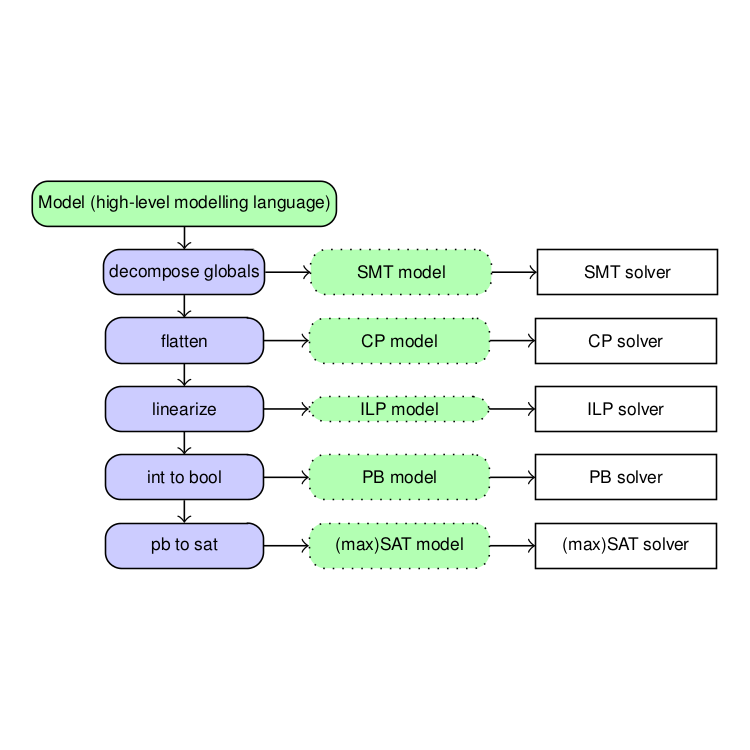
\includegraphics[height=30mm, trim=30px 30px 30px 30px, clip]{images/ch6-logo.png}
	\end{center}
	
	\vspace{-1em}
	Better understand what a solver CAN do, and what it is GOOD at (or bad).
	\begin{itemize}
		\item SAT: recommended if very Boolean
		\item PB: recommended if very Boolean but also many linear sums
		\item ILP: recommended if many linear constraints and optimizing the 'continuous relaxation' is meaningful
		\item SMT: recommended if many disjunctive constraints (SAT reasoning + LIA reasoning)
		\item CP: recommended if you have many global constraints
	\end{itemize}
	
	
	(but there is no rulebook)
\end{frame}

\iffalse
\begin{frame}{Choosing a Solver Technology}
  \begin{itemize}
    \item Do you need guarantees that a found solution is optimal, \\
      that all solutions are found, and that unsatisfiability is
      provable? \vfill
    \item What types of decision variables are in your model? \vfill
    \item What constraint predicates are in your model? \vfill
    \item Does your problem look like a well-known problem? \vfill
    \item How do backends perform on easy problem instances? \vfill
    \item What is your favourite technology or backend?
  \end{itemize}
\end{frame}
\fi

\begin{frame}{Some Caveats}
  \begin{itemize}
    \item Each problem can be modelled in many different ways.
    \item Different models of the same problem are better suited for different
      backends.
    \item Performance on small instances does not always scale to larger
      instances.
    \item Sometimes, a good \search{search strategy} is more important
      than a good model.
    \item Not all backends of the same technology have comparable
      performance.
    \item Some pure problems can be solved by specialist solvers, \\
      such as
      \href{https://www.math.uwaterloo.ca/tsp/concorde}{Concorde} for
      the travelling salesperson problem, \\ but real-life side
      constraints often make them inapplicable.
    %\item Some problems are maybe even solvable in polynomial time and
      space.
  \end{itemize}
\end{frame}

\begin{frame}
  \structured{Take-Home Message:}
  \begin{itemize}
    \item There are many solving technologies and ways to encode to them.
    \item It is useful to understand the commonalities and differences.
    \item No solving technology can be universally better
      than all the others, unless $\textnormal{P} = \textnormal{NP}$.
  \end{itemize}
  \begin{center}
    \handpoint\ With solver-independent frameworks: can try multiple ones!
  \end{center}

\end{frame}

\end{document}
